This test problem uses a time-independent manufactured solution to isolate
spatial errors: $\scalarsolution(x)=\sin(\pi x)$. The problem summary is
given in Table \ref{tab:mms_sinx_ss}.

%-------------------------------------------------------------------------------
\begin{table}[htb]\caption{Convergence Test Problem 1 Summary}
\label{tab:mms_sinx_ss}
\centering
\begin{tabular}{l l}\toprule
\emph{Parameter} & \emph{Value}\\\midrule
Domain & $\mathcal{D} = (0,1)$\\
Boundary Conditions & $\scalarsolution(x)=0,\quad x\in\partial\mathcal{D}^-$,\\
   & $\quad\partial\mathcal{D}^-=\{x\in\partial\mathcal{D}:\mathbf{n}(x)
       \cdot\mathbf{\Omega}<0\}$\\
Direction & $\mathbf{\Omega} = \mathbf{e}_x$\\
Cross Section & $\reactioncoef(x)=1$\\
Source & $\scalarsource(x)=\pi\cos(\pi x) + \sin(\pi x)$\\
Speed & $\speed=1$\\
Exact Solution & $\scalarsolution(x)=\sin(\pi x)$\\
\bottomrule\end{tabular}
\end{table}
%-------------------------------------------------------------------------------

This problem was run in steady-state to avoid temporal error so that spatial
convergence rates could accurately be measured.
The coarsest mesh size in this study uses 8 cells, and each successive mesh
size is halved, with the finest mesh in the study using 256 cells.

Figure \ref{fig:mms_sinx_ss_solution} shows a comparison of the solutions with
32 cells, and Figure \ref{fig:mms_sinx_ss_visc} compares the viscosity
profiles. Only the low-order (DMP) method does not match the exact solution
well and suffers a defect at the outflow (right) boundary.
The entropy viscosity and Galerkin FCT methods use the analytic solution bounds
given by Equation \eqref{eq:analyticDMP_ss} with the antidiffusion bounds fix given by
Equation \eqref{eq:antidiffusion_bounds_operation}:
\[
  \tilde{\antidiffusionbound}_i^-
    \equiv \min(\antidiffusionbound_i^-, 0)
  \eqc
\]
\[
  \tilde{\antidiffusionbound}_i^+
    \equiv \max(\antidiffusionbound_i^+, 0)
  \eqp
\]
Since in the steady-state
case the FCT solution bounds are implicit, the system is nonlinear and requires
iteration. To produce the results that follow, the high-order solution was
used as the initial guess in this iteration. It should be noted that for this
test problem, using other guesses, such as zero or the low-order solution,
leads to serious nonlinear convergence issues, for which a remedy is not
currently known.

%-------------------------------------------------------------------------------
\begin{figure}[ht]
   \centering
      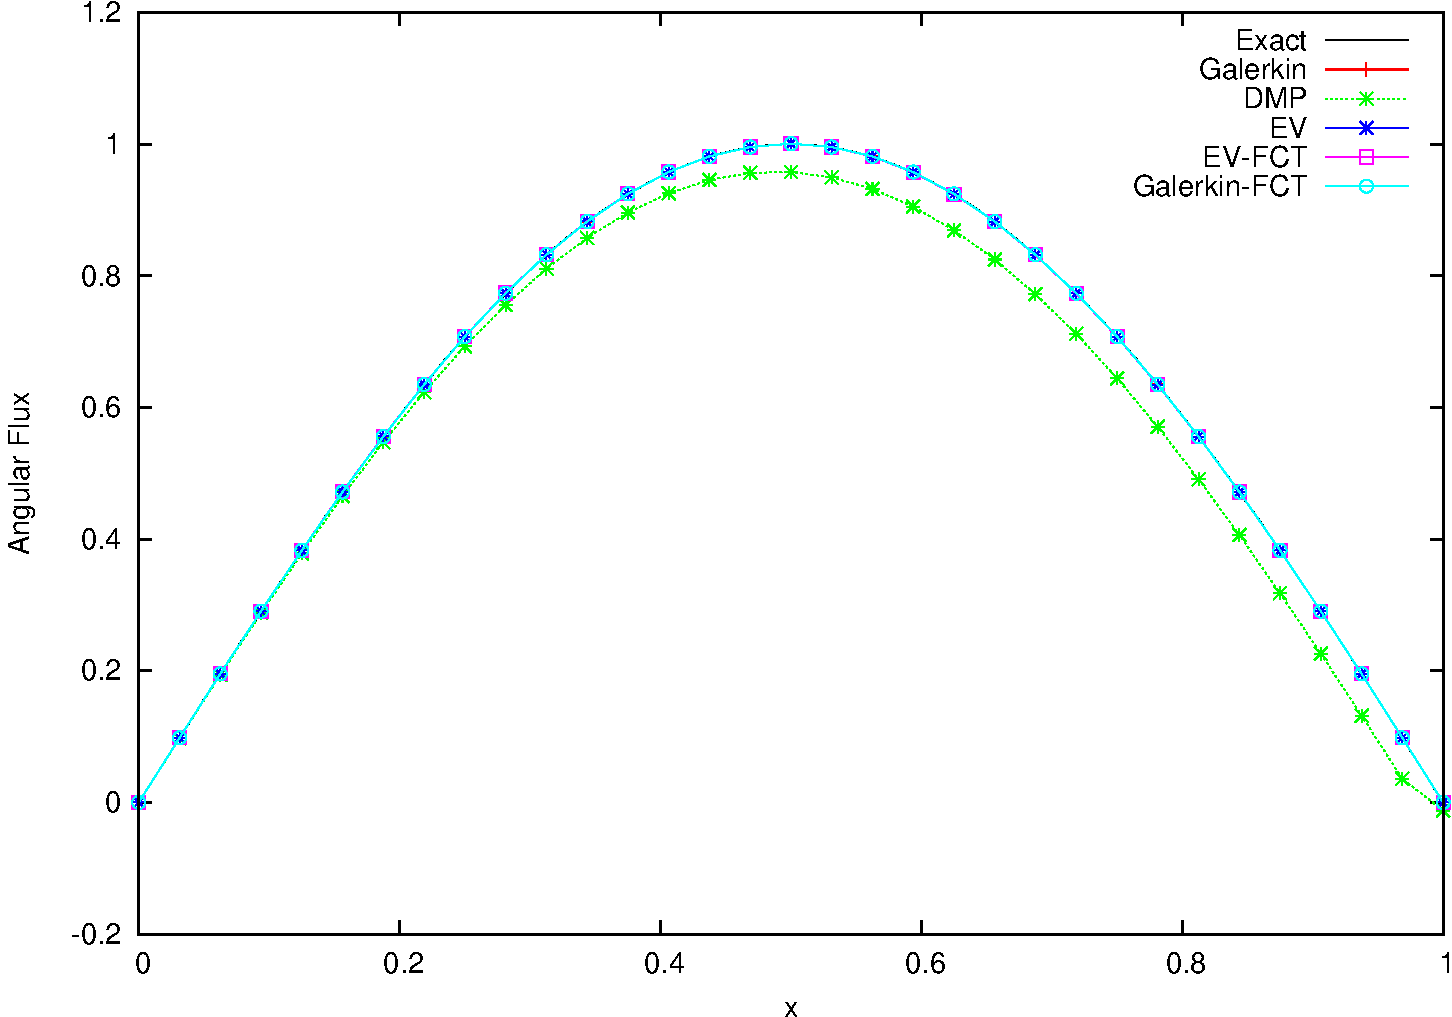
\includegraphics[width=\textwidth]
        {\contentdir/results/transport/mms_sinx_ss/images/solution.pdf}
      \caption{Comparison of Solutions for Convergence Test Problem 1 with 32 Cells}
   \label{fig:mms_sinx_ss_solution}
\end{figure}
%-------------------------------------------------------------------------------
%-------------------------------------------------------------------------------
\begin{figure}[ht]
   \centering
      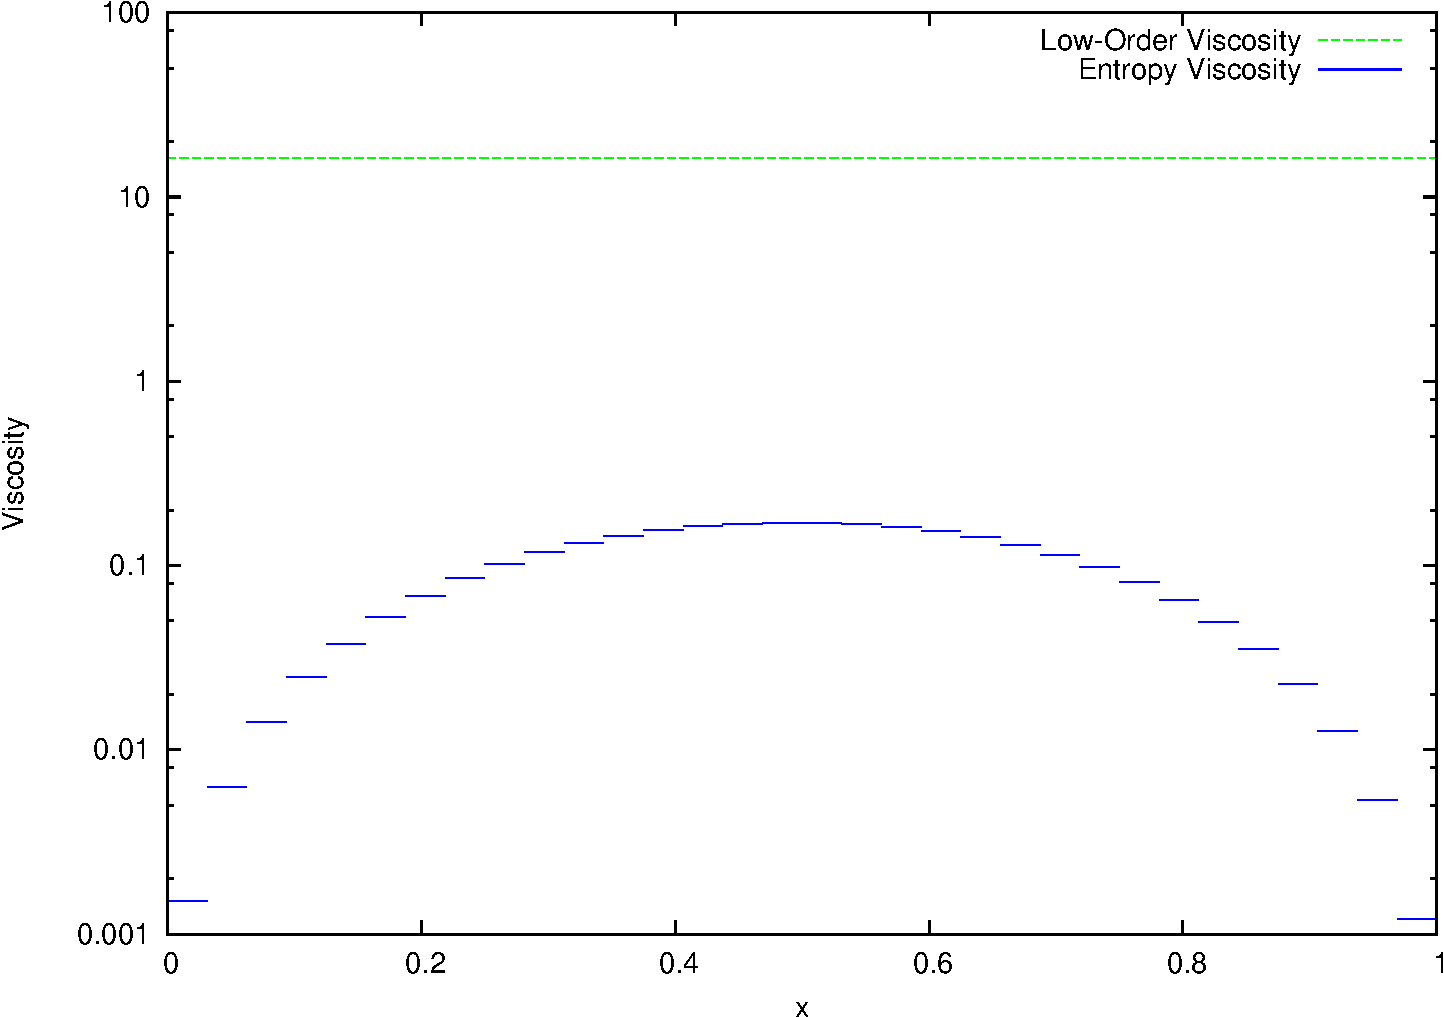
\includegraphics[width=\textwidth]
        {\contentdir/results/transport/mms_sinx_ss/images/viscosity_SS.pdf}
      \caption{Viscosity Profiles for Convergence Test Problem 1 with 32 Cells}
   \label{fig:mms_sinx_ss_visc}
\end{figure}
%-------------------------------------------------------------------------------

Figure \ref{fig:mms_sinx_ss_convergence} shows a comparison of
errors with different methods. The DMP low-order method achieves first-order
spatial convergence as expected, and all other methods achieve second-order
spatial convergence. The entropy viscosity method and the FCT method employing
it both start with more error for the coarsest mesh than the Galerkin method,
but upon refinement, the differences in error diminish.

%-------------------------------------------------------------------------------
\begin{figure}[ht]
   \centering
      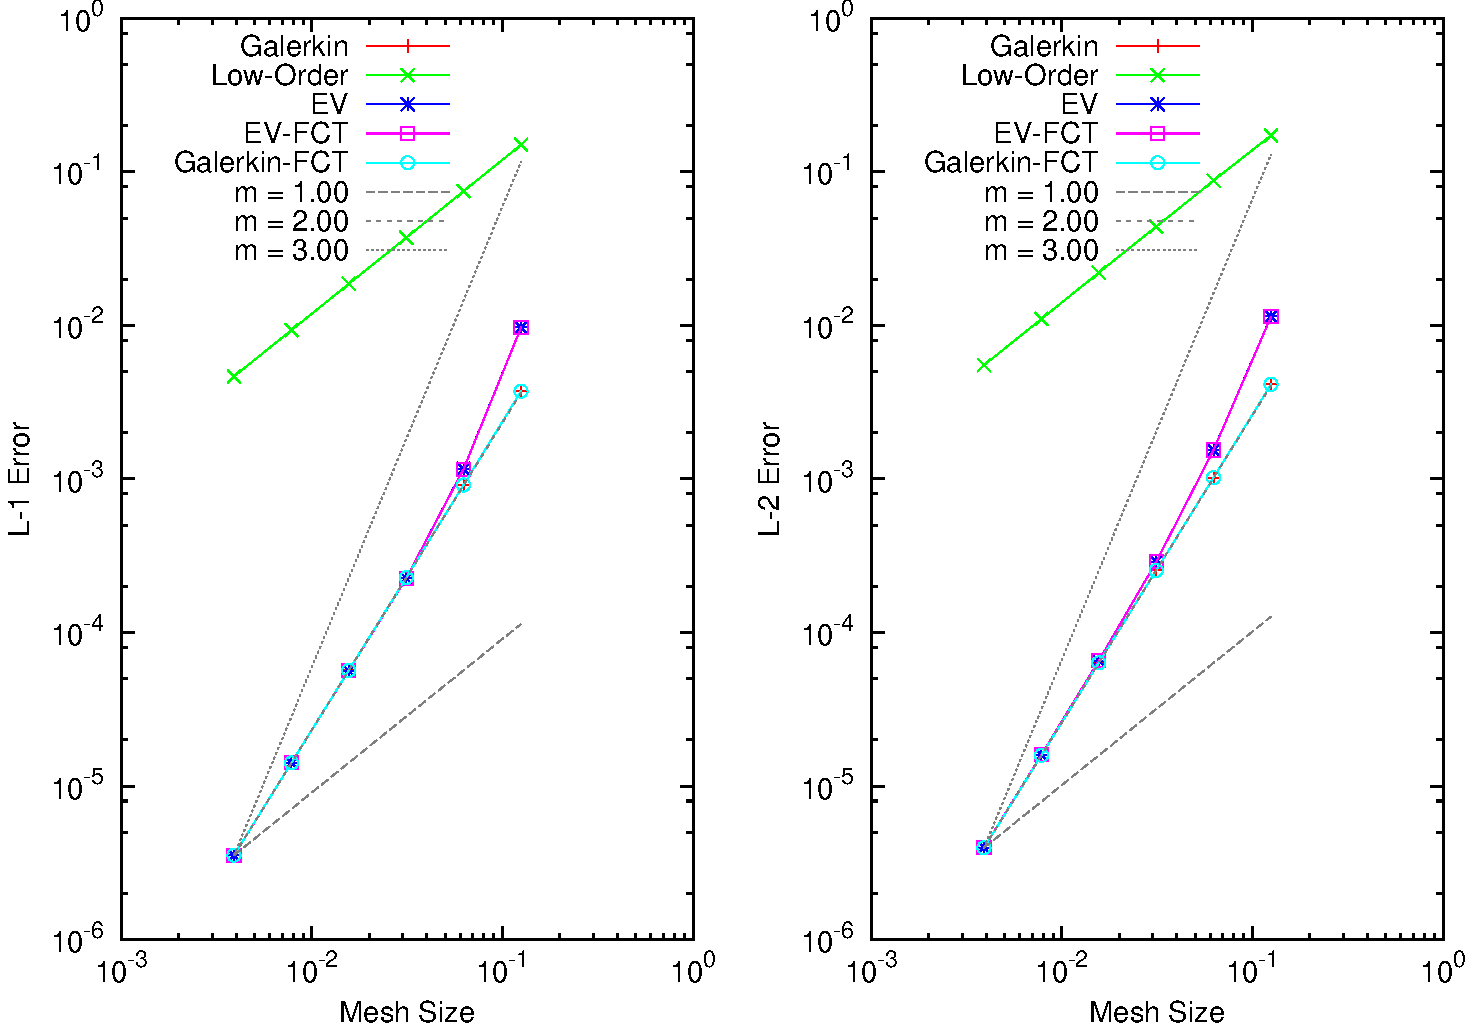
\includegraphics[width=\textwidth]
        {\contentdir/results/transport/mms_sinx_ss/images/convergence.pdf}
      \caption{Comparison of Errors for Convergence Test Problem 1}
   \label{fig:mms_sinx_ss_convergence}
\end{figure}
%-------------------------------------------------------------------------------

If the FCT methods use the low-order discrete maximum principle
expressions given by Equation \eqref{eq:DMP_ss} as solution bounds instead
of the analytic solution bounds, then results are much different for the
FCT schemes. Figure \ref{fig:mms_sinx_ss_solution_vs} shows a comparison
of the entropy viscosity FCT solutions with 32 cells using the analytic bounds vs. using
the low-order DMP bounds, and Figure \ref{fig:mms_sinx_ss_convergence_vs}
shows a comparison of the errors. For this test problem, using the low-order
DMP for the FCT solution bounds results in reducing the FCT solution to the low-order
solution. From this example it is evident that the selection of solution
bounds is critical to the success of the FCT algorithm.

%-------------------------------------------------------------------------------
\begin{figure}[ht]
   \centering
      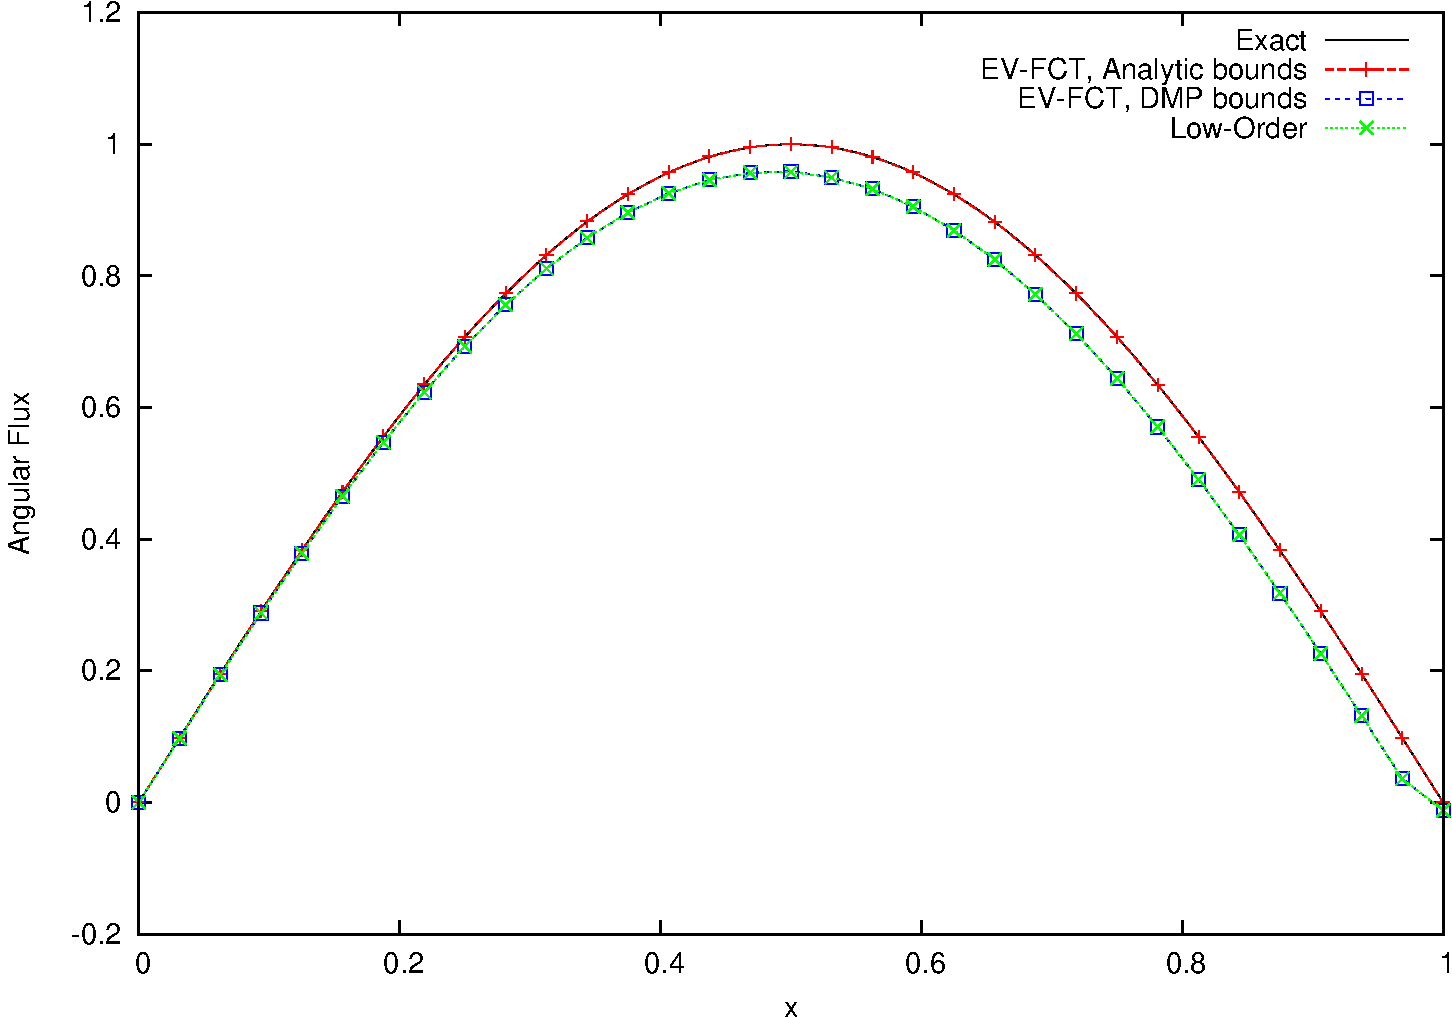
\includegraphics[width=\textwidth]
        {\contentdir/results/transport/mms_sinx_ss/images/solution_analytic_vs_dmp.pdf}
      \caption{Comparison of FCT Solutions with Different Solution Bounds with 32 Cells}
   \label{fig:mms_sinx_ss_solution_vs}
\end{figure}
%-------------------------------------------------------------------------------
%-------------------------------------------------------------------------------
\begin{figure}[ht]
   \centering
      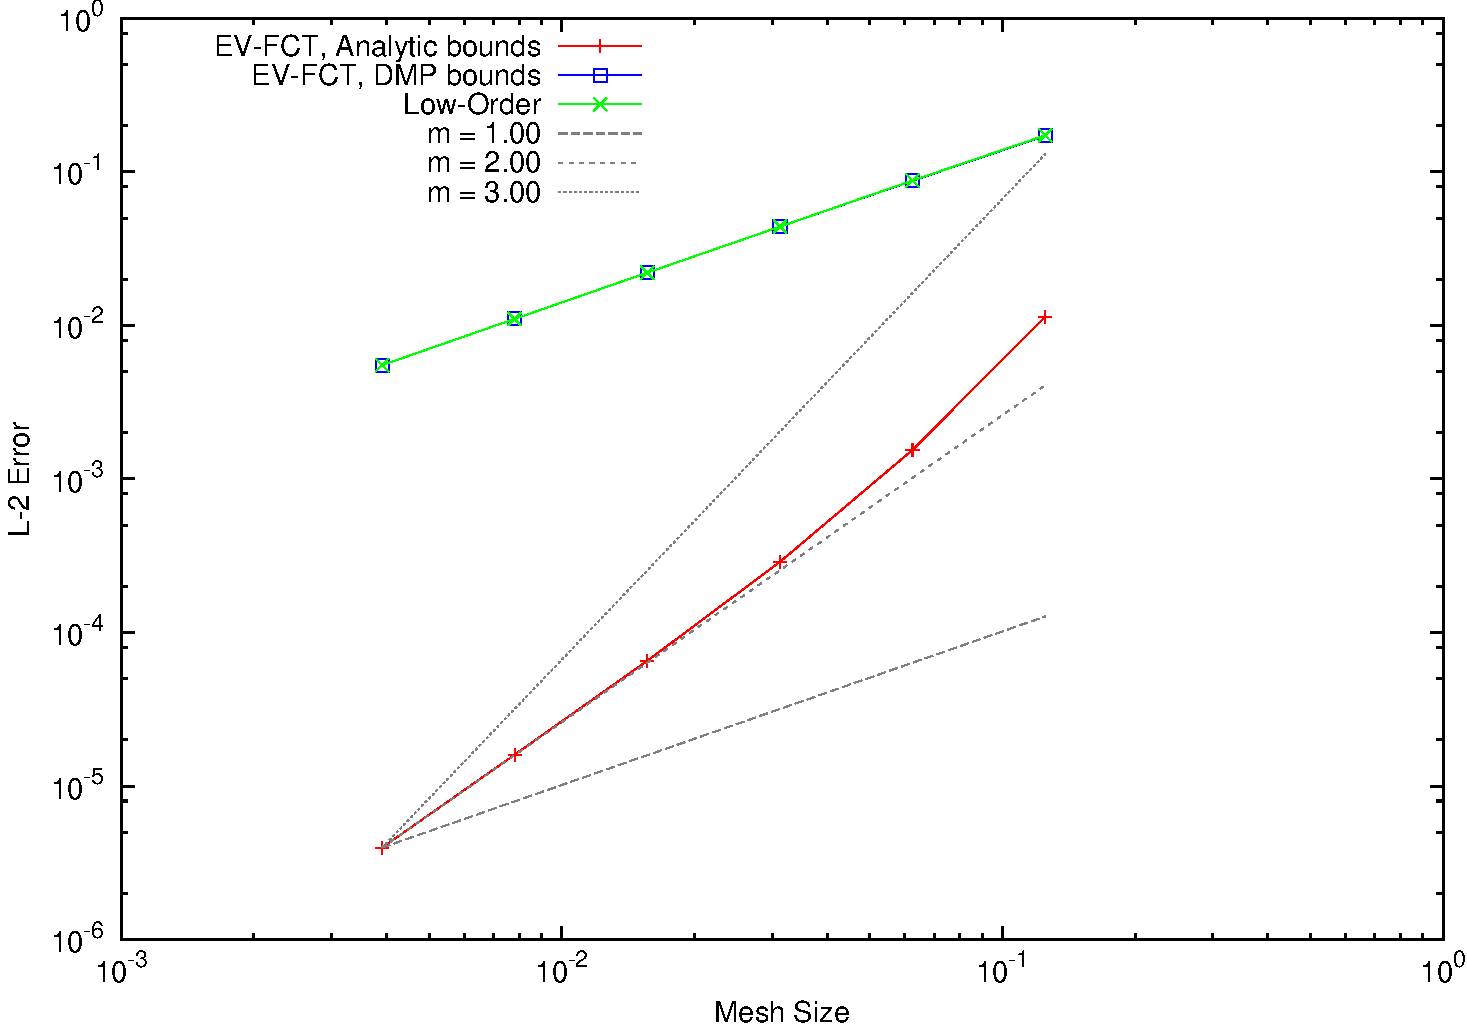
\includegraphics[width=\textwidth]
        {\contentdir/results/transport/mms_sinx_ss/images/convergence_analytic_vs_dmp.pdf}
      \caption{Comparison of Error of FCT Solutions with Different Solution Bounds}
   \label{fig:mms_sinx_ss_convergence_vs}
\end{figure}
%-------------------------------------------------------------------------------
\clearpage
